\documentclass[10pt]{article}
\usepackage{icmlko}

\icmlmeta{IP 파운데이션 월드모델}{331}{모형 밑의 바닥}{배깅을 세 배 해도 아이돌은 10\%밖에 안 준다 --- 흔들림의 72\%가 자료다}

\begin{document}

\twocolumn[
\icmlheader

\begin{abstract}
노트 330이 ``챔피언이 제일 작은 도메인에서 3$\sim$4배 흔들린다''를 남기고
``배깅을 늘리면 되나''를 갈래로 뒀다. \textbf{쟀다} --- $K{=}8$ 과
$K{=}24$ 를 같은 학습 재추출 뽑기 열둘에서 짝지어 돌렸다.

\textbf{판은 못 가른다}: 짝지은 차 $+$0.0023(SD 0.0048 · 9/12 양수)로
미결정 폭 0.010 안이다. \textbf{비용은 세 배다.}

\textbf{흔들림은 도메인마다 다르게 준다.} 배깅이 줄이는 것은 \emph{모형}
분산뿐이므로 $\mathrm{SD}_K^2 = V_{\text{자료}} + V_{\text{모형}}/K$ 로
두 몫을 가를 수 있다. $K$ 를 세 배 해서 SD 가 42\% 줄면 전부 모형 몫이고
0\% 줄면 전부 자료 몫이다.

\begin{center}\footnotesize
\begin{tabular}{lrrr}
\hline
도메인 & 유보 & 준 것 & 모형 몫 \\
\hline
\textbf{시장팝업} & 104 & \textbf{$-$37\%} & \textbf{90\%} \\
\textbf{펀딩} & 80 & \textbf{$-$36\%} & \textbf{89\%} \\
팝업 & 59 & $-$18\% & 49\% \\
\textbf{아이돌} & 25 & $-$10\% & \textbf{28\%} \\
게임 · 세계애니 & 180 · 300 & $-$8\% & 24\% \\
애니 · 웹툰 & 606 · 711 & $-$7\% & 16$\sim$20\% \\
모바일 · 도서 & 441 · 163 & $+$7 · $+$13\% & 0\% \\
\hline
\end{tabular}
\end{center}

\textbf{두 자리에서는 배깅이 크게 산다}(시장팝업 · 펀딩 --- 모형 몫이
90\%다). \textbf{그런데 제일 아픈 자리에서는 안 산다} --- 아이돌은 모형
몫이 28\% 뿐이라 $K$ 를 무한대로 보내도 SD 가 0.1277 에서 \textbf{0.1081}
까지밖에 안 내려간다. \textbf{나머지 72\%는 자료다.}

\textbf{그래서 노트 325$\sim$331이 한 바퀴를 돈다.} 아이돌을 못 재는 것은
모형 문제가 아니다. \textbf{행이 없어서다.} 노트 326이 찾은 94행 ---
그리고 그 행들을 쓰려면 위키와 앨범 메타를 긁어야 한다는 것 --- 이
바닥을 내리는 유일한 길이다.
\end{abstract}
]

\section{배깅이 줄이는 것}

\texttt{F18\_bagboost} 는 부스팅을 부트스트랩으로 $K{=}8$ 번 적합해 순위를
평균한다. 배깅은 \textbf{주어진 학습 자료 안에서} 생기는 분산을 줄인다 ---
자료 자체가 다른 뽑기였다면 어땠을까는 못 줄인다.

\[ \mathrm{SD}_K^2 \;=\; V_{\text{자료}} \;+\; V_{\text{모형}}/K \]

$K{=}8$ 과 $K{=}24$ 를 재면 두 몫이 갈린다. \textbf{미리 적었다}(전등록
\texttt{preregister\_bagk.json}) --- ``배깅은 주어진 학습 자료 안에서의
분산을 줄인다. 학습 자료 자체가 바뀌는 분산은 안 줄 수 있다. 그럴 가능성이
반이라고 미리 적는다.''

\begin{figure*}[t]
\centering
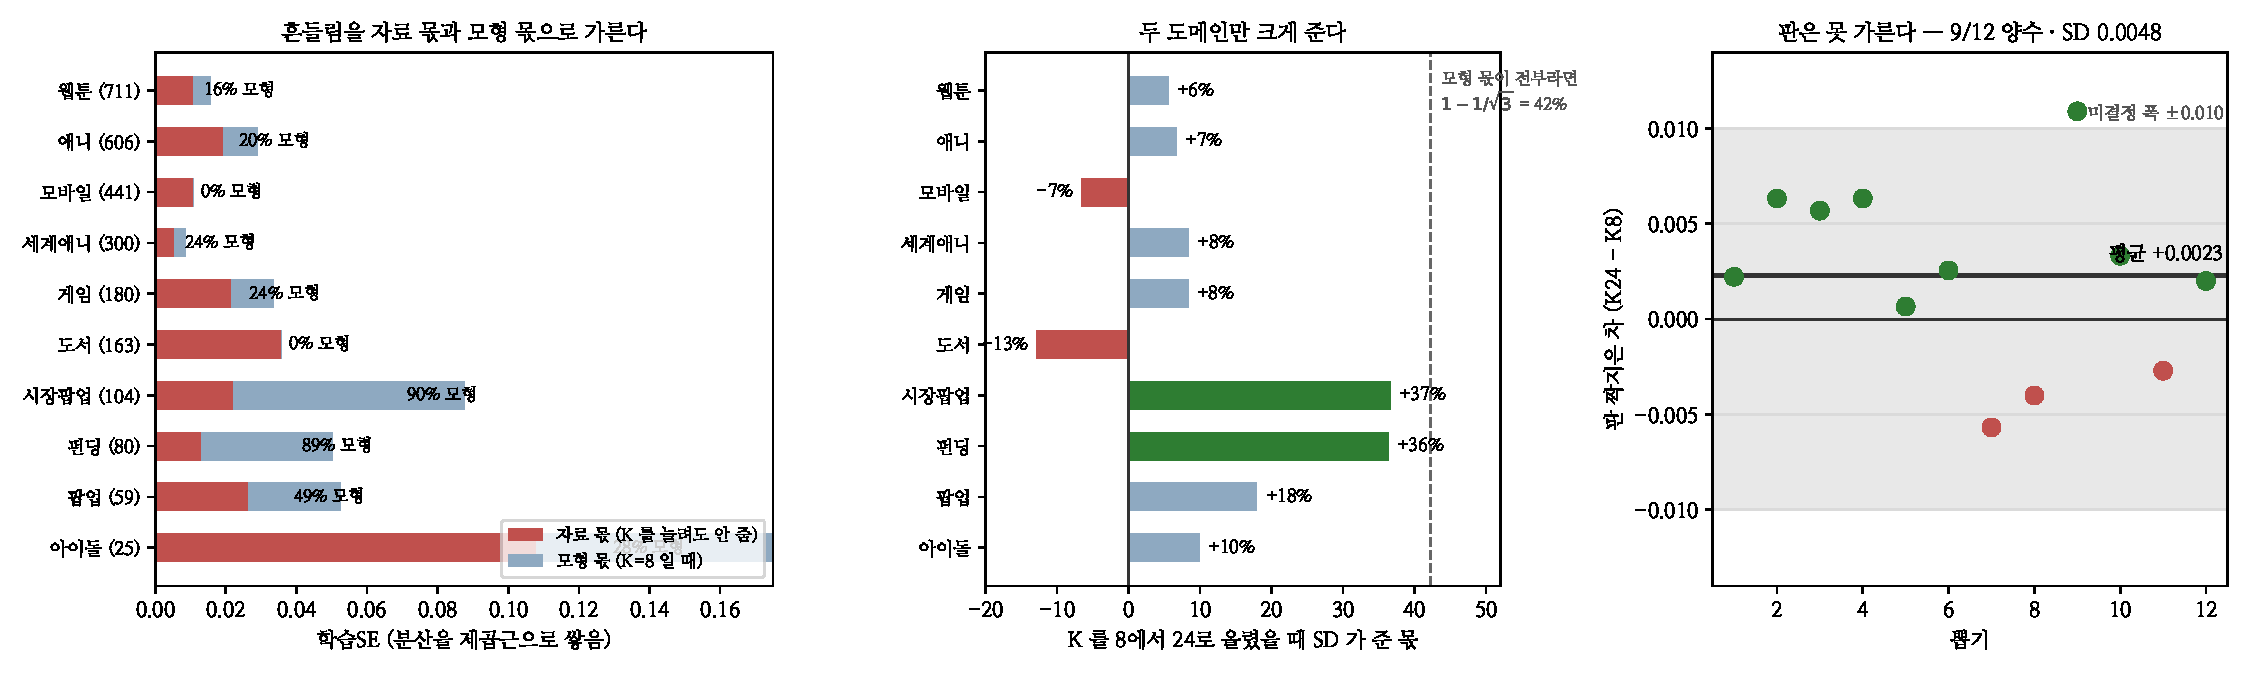
\includegraphics[width=\textwidth]{figs/bagk.pdf}
\caption{왼쪽 --- 자료 몫과 모형 몫. 가운데 --- $K$ 를 세 배 했을 때
SD 가 준 몫. 오른쪽 --- 판 짝지은 차.}
\end{figure*}

\section{판은 못 가른다}

\begin{center}\small
\begin{tabular}{lrr}
\hline
 & $K{=}8$ & $K{=}24$ \\
\hline
기준 판 & 0.4681 & 0.4756 \\
판 학습SE & 0.0041 & 0.0066 \\
\hline
\multicolumn{3}{l}{짝지은 차 $+$0.0023 · SD 0.0048 · 9/12 양수} \\
\multicolumn{3}{l}{미결정 폭 0.010 안 --- \textbf{못 가른다}} \\
\hline
\end{tabular}
\end{center}

\textbf{비용이 세 배인데 판이 안 움직인다.} 그리고 노트 329의 규약대로
자료를 안 바꾸는 처치이므로 판 판정이 그대로 적용된다.

\section{두 몫}

\begin{center}\footnotesize
\begin{tabular}{lrrrr}
\hline
도메인 & 유보 & SD($K$8) & 자료 SD & 모형 몫 \\
\hline
웹툰 & 711 & 0.0118 & 0.0108 & 16\% \\
애니 & 606 & 0.0217 & 0.0195 & 20\% \\
모바일 & 441 & 0.0108 & 0.0108 & 0\% \\
세계애니 & 300 & 0.0064 & 0.0055 & 24\% \\
게임 & 180 & 0.0246 & 0.0215 & 24\% \\
도서 & 163 & 0.0358 & 0.0358 & 0\% \\
\textbf{시장팝업} & 104 & 0.0692 & \textbf{0.0222} & \textbf{90\%} \\
\textbf{펀딩} & 80 & 0.0395 & \textbf{0.0130} & \textbf{89\%} \\
팝업 & 59 & 0.0372 & 0.0265 & 49\% \\
\textbf{아이돌} & 25 & 0.1277 & \textbf{0.1081} & 28\% \\
\hline
\end{tabular}
\end{center}

\paragraph{시장팝업과 펀딩은 배깅으로 산다} 둘 다 모형 몫이 90\% 다.
$K$ 를 세 배 하니 SD 가 각각 37\% · 36\% 줄었다 --- 이론 상한 42\% 에
가깝다. \textbf{이 둘은 흔들림이 자료 부족이 아니라 나무의 변덕이었다.}

\paragraph{아이돌은 안 산다} 모형 몫 28\%. $K \to \infty$ 라도 SD 가
0.1081 이다. 노트 327의 위약 SD 0.0922 · 노트 330의 학습SE 0.1093 과
같은 자리를 가리킨다 --- \textbf{아이돌은 어떤 추정기 장치로도 이 아래로
못 간다.}

\paragraph{경고} 뽑기 열둘이라 SD 추정의 SE 가 21\% 다. 모바일 · 도서는
$K{=}24$ 의 SD 가 더 커서 모형 몫이 음수로 나와 0 으로 잘랐다 ---
\textbf{그 둘은 ``모형 몫이 작다''로만 읽어야 한다.} 시장팝업 · 펀딩의
90\% 는 감소폭이 커서 잡음으로 설명하기 어렵지만, 다시 재기 전까지는
\textbf{가리키는 방향}으로만 쓴다.

\section{한 바퀴가 닫힌다}

\begin{center}\footnotesize
\begin{tabular}{ll}
\hline
노트 & 무엇 \\
\hline
325 & 아이돌 94행이 안 쓰인다 --- 라벨 기준 때문인 줄 \\
326 & 아니다. \textbf{풀 안쪽만 긁어서}다 \\
327 & 넣으면 $+$0.0881 인데 위약 SD 가 0.092 다 \\
330 & 학습SE 0.1093 --- 정식화마다 3$\sim$4배 \\
\textbf{331} & \textbf{72\%가 자료다 --- 모형으로는 못 내린다} \\
\hline
\end{tabular}
\end{center}

\textbf{아이돌을 못 재는 것은 모형 문제가 아니다.} $K$ 를 올려도 · 정식화를
바꿔도(F10 이 0.0292 지만 그건 예측을 평평하게 만들어 얻은 것이다) 바닥이
안 내려간다. \textbf{행이 없어서다.} 유보 25행 · 학습 54행.

\section{남은 것}
\begin{center}\footnotesize
\begin{tabular}{ll}
\hline
갈래 & 왜 \\
\hline
\textbf{시장팝업 · 펀딩만 $K$ 를} & 그 둘만 모형 몫 90\% \\
도메인마다 다른 $K$ & 판은 그대로, 흔들림만 준다 \\
아이돌 94행 위키 · 앨범 긁기 & \textbf{바닥을 내리는 유일한 길} \\
씨앗 평균은 얼마나 주나 & 공식 판은 씨앗 셋을 평균한다 \\
\hline
\end{tabular}
\end{center}

\paragraph{규약} \textbf{장치로 못 내리는 바닥이 있다.} 배깅 · 수축 ·
씨앗 평균은 다 \emph{모형} 분산을 다루는 장치인데, 작은 도메인의 흔들림은
대부분 \emph{자료} 분산이다. \textbf{그리고 그 둘은 겉보기에 안 갈린다}
--- 둘 다 ``SE''라는 한 수로 나온다. $K$ 를 바꿔 보는 것이 가르는 제일 싼
방법이었다. \textbf{어떤 수치가 안 좋을 때 모형을 손보기 전에 그 수치의
몇 퍼센트가 모형 몫인지부터 재라} --- 아이돌은 28\% 였고, 세 배를 들여
10\% 를 얻었다.

\end{document}
